\documentclass[10pt,twocolumn,letterpaper]{article}

\usepackage{cvpr}
\usepackage{times}
\usepackage{epsfig}
\usepackage{graphicx}
\usepackage{amsmath}
\usepackage{amssymb}

% Include other packages here, before hyperref.
\usepackage{cite}
\usepackage{ctable}
\usepackage{hhline}
\usepackage{booktabs}
\usepackage{subcaption}
\usepackage{csquotes }

\newcolumntype{L}[1]{>{\raggedright\let\newline\\\arraybackslash\hspace{0pt}}m{#1}}
\newcolumntype{C}[1]{>{\centering\let\newline\\\arraybackslash\hspace{0pt}}m{#1}}
\newcolumntype{R}[1]{>{\raggedleft\let\newline\\\arraybackslash\hspace{0pt}}m{#1}}

% If you comment hyperref and then uncomment it, you should delete
% egpaper.aux before re-running latex.  (Or just hit 'q' on the first latex
% run, let it finish, and you should be clear).
\usepackage[breaklinks=true,bookmarks=false]{hyperref}

\cvprfinalcopy % *** Uncomment this line for the final submission

\def\cvprPaperID{****} % *** Enter the CVPR Paper ID here
\def\httilde{\mbox{\tt\raisebox{-.5ex}{\symbol{126}}}}

% Pages are numbered in submission mode, and unnumbered in camera-ready
%\ifcvprfinal\pagestyle{empty}\fi
\ifcvprfinal\pagestyle{empty}\fi
\begin{document}

%%%%%%%%% TITLE
\title{V2V-PoseNet: Voxel-to-Voxel Prediction Network for Accurate 3D Hand and Human Pose Estimation from a Single Depth Map}

\author{Gyeongsik Moon\\
Department of ECE, ASRI\\
Seoul National University\\
{\tt\small mks0601@snu.ac.kr}
% For a paper whose authors are all at the same institution,
% omit the following lines up until the closing ``}''.
% Additional authors and addresses can be added with ``\and'',
% just like the second author.
% To save space, use either the email address or home page, not both
\and
Ju Yong Chang\\
Department of EI\\
Kwangwoon University\\
{\tt\small juyong.chang@gmail.com}
\and
Kyoung Mu Lee\\
Department of ECE, ASRI\\
Seoul National University\\
{\tt\small kyoungmu@snu.ac.kr}
}

\maketitle
%\thispagestyle{empty}

%%%%%%%%% ABSTRACT
\begin{abstract}
Most of the existing deep learning-based methods for 3D hand and human pose estimation from a single depth map are based on a common framework that takes a 2D depth map and directly regresses the 3D coordinates of keypoints, such as hand or human body joints, via 2D convolutional neural networks (CNNs). The first weakness of this approach is the presence of perspective distortion in the 2D depth map. While the depth map is intrinsically 3D data, many previous methods treat depth maps as 2D images that can distort the shape of the actual object through projection from 3D to 2D space. This compels the network to perform perspective distortion-invariant estimation. The second weakness of the conventional approach is that directly regressing 3D coordinates from a 2D image is a highly non-linear mapping, which causes difficulty in the learning procedure. To overcome these weaknesses, we firstly cast the 3D hand and human pose estimation problem from a single depth map into a voxel-to-voxel prediction that uses a 3D voxelized grid and estimates the per-voxel likelihood for each keypoint. We design our model as a 3D CNN that provides accurate estimates while running in real-time. Our system outperforms previous methods in almost all publicly available 3D hand and human pose estimation datasets and placed first in the HANDS 2017 frame-based 3D hand pose estimation challenge. The code is available in \footnote{\url{https://github.com/mks0601/V2V-PoseNet_RELEASE}}.
\end{abstract}

%%%%%%%%% BODY TEXT
\section{Introduction}

Locating visual landmarks, such as human body joints \cite{toshev2014deeppose} and facial key points \cite{xiong2013supervised}, is an important yet challenging problem. The stacked U-Nets, {\it e.g.} hourglasses (HGs) \cite{newell2016stacked}, are widely used in landmark localization. Generally speaking, their success can be attributed to design patterns: 1) within each U-Net, connect the top-down and bottom-up feature blocks to encourage gradient flow; and 2) stack multiple U-Nets in a cascade to refine prediction stage by stage.

However, the shortcut connection exists only ``locally'' inside each U-Net \cite{ronneberger2015u}. There is no ``global'' connection across U-Nets except the cascade. Blocks in different U-Nets cannot share features, which may impede the information flow and lead to redundant parameters.

We propose densely connected U-Nets (DU-Net) to address this issue. The key idea is to directly connect blocks of the same semantic meanings, {\it i.e.} having the same resolution in either top-down or bottom-up context, from any U-Net to all subsequent U-Nets. Please refer to Fig. \ref{fig:framework} for an illustration. The dense connectivity is similar to DenseNet \cite{huang2016densely} but generalizing the design philosophy from feature to semantic level. It encourages information flow as well as feature reuse ``globally'' across the stacked U-Nets, yielding improved localization accuracy. 

Yet there are critical issues in designing DU-Net: 1) The number of parameters would have a quadratic growth since $n$ stacked U-Nets could generate $O(n^2)$ connections. 2) A naive implementation may allocate new memory for every connection, making the training highly expensive and limiting the maximum depth of DU-Nets. 

% The training would be extremely memory expensive since a naive implementation has to make a copy of every connected feature for network forward and back propagation.  



\begin{figure*}[t!]
\centering
  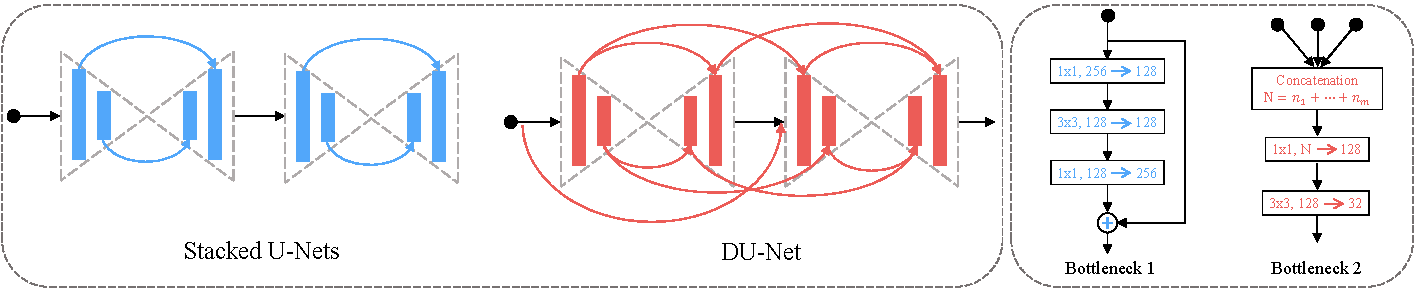
\includegraphics[width=1.0\linewidth]{figures/framework-cropped.pdf}
\caption{Illustration of stacked U-Nets and DU-Net. Stacked U-Nets has skip connections only within each U-Net. In contrast, DU-Net also connects blocks with the same semantic meanings across different U-Nets. The feature reuse could significantly reduce the size of bottleneck in each block, as shown in the right figure. Consequently, with the same number of U-Nets, DU-Net has only 30\% parameters of stacked U-Nets.}
\label{fig:framework}
\end{figure*}

% 
Our solution to those efficiency issues is threefold. {\bf First}, instead of connecting all stacked U-Nets, we only connect a U-Net to its $K$ successors. We name it as the $order$-$K$ connectivity, which aims to balance the fitting accuracy and parameter efficiency by cutting off long-distance connections. {\bf Second}, we employ a memory-efficient implementation in training. The key idea is to reuse a pre-allocated memory so all connected blocks could share the same memory. Compared with the naive implementation, this strategy makes it possible to train a very deep DU-Net (actually, $2\times$ deeper). {\bf Third}, to further improve the efficiency, we investigate an iterative design that may reduce the model size to one half. More specifically, the output of the first pass of the DU-Net is used as the input of the second pass, where detection or regression loss is applied as supervision. 

% %G%
% In view of deploying our approach on mobile devices, we further attempt to quantize weights, inputs, and gradients of DU-Net to low bit-width discrete values. This not only decreases the high precision operations but also shrinks the memory usage during training. By network quantization, the size of trained model can also be largely compressed.
% %G%
Besides shrinking the number of network parameters, we also study to further quantize each parameter. This motivates from the ubiquitous mobile applications. Although current mobile devices could carry models of dozens of MBs, deploying such networks requires high-end GPUs. However, quantized models could be accelerated by some specifically designed low-cost hardwares. Beyond only deploying models on mobile devices \cite{li2017deeprebirth}, training deep neural networks on distributed mobile devices emerges recently \cite{mcmahan2016communication}. To this end, we also try to quantize not only the model parameters but also its inputs (intermediate features) and gradients in training. This is the first attempt to investigate training landmark localizers using quantized inputs and gradients.


In summary, our key contributions are:
\begin{itemize}
    \item To the best of our knowledge, we are the first to propose quantized densely connected U-Nets for visual landmark localization, which largely improves the information flow and feature reuse at the semantic level.
    \item We propose the $order$-$K$ connectivity to balance accuracy and efficiency. It decreases the growth of model size from quadratic to linear by removing trivial connections. Experiments show it could reduce $\sim$70\% parameters of state-of-the-art landmark localizers.
    \item Very deep U-Nets can be trained using a memory-efficient implementation, where pre-allocated memory is reused by all connected blocks.
    \item We further investigate an iterative refinement that may cut down half of the model size, by forwarding DU-Net twice using either detection or regression supervision.
    %G%
    \item Different from previous efforts of quantizing only the model parameters, we are the first to quantize their inputs and gradients for better training efficiency on landmark localization tasks. By choosing appropriate quantization bit-widths for weights, inputs and gradients, quantized DU-Net achieves $\sim$75\% training memory saving with comparable performance. 
    %G%
    \item Exhaustive experiments are performed to validate DU-Net in different aspects. In both human pose estimation and face alignment, DU-Net demonstrates comparable localization accuracy and use $\sim$2\% model size compared with state-of-the-art methods.
\end{itemize}

% We are the first to deploy network quantization for better training efficiency on localization tasks. By choosing appropriate quantization bit-widths for weights, inputs and gradients, quantized DU-Net achieves at least 32$\times$ memory saving with comparable performance to the-state-of-art approaches. 


%The landmark localization such as human pose estimation \cite{toshev2014deeppose,newell2016stacked,wei2016convolutional}, facial landmark localization \cite{xiong2013supervised,zhang2014facial,sagonas2013300}, etc, plays an important role in the higher-level image understanding. The Convolutional Neural Networks (CNNs) have dominated this field, among which recent architecture of stacked hourglasses \cite{newell2016stacked}, a variant of the U-Net \cite{ronneberger2015unet}, becomes a standard solution. The skip connections between top-down and bottom-up blocks within a U-Net could preserve the spatial information and increase the gradient flow. With multiple U-Nets stacked together, the prediction could be refined stage by stage. However, the connections are only within each U-Net of the stacked hourglasses and no explicit connections exist between U-Nets, which may impede the information flow across them. And the blocks with the same semantics in different U-Nets cannot share features, leading to many redundant parameters. 

% Its success attributes to three key factors: repeated top-down, bottom-up inferences, intermediate supervisions and residual bottlenecks \cite{}. 

% The multiple stage top-down and bottom-up processing could better integrate both the local and global visual contexts into the final prediction. The intermediate supervision and residual bottlenecks, on the other hand, could alleviate the gradient vanish problem in deep networks.
%In this paper, we propose to densely connect stacked U-Nets by linking blocks with the same semantics in different U-Nets. We refer to this architecture as {\it Dense U-Nets}. The blocks in a U-Net could get direct inputs from its connected blocks in all preceding U-Nets, making the information flow more efficiently among the U-Nets. The feature reuse at each resolution could reduce the parameters in each block. The dense connectivity in our Dense U-Nets is different from that of DenseNet \cite{huang2016densely}. More specifically, layers only within each single block of the DenseNet are connected. In contrast, we connect blocks lying across the whole Dense U-Nets and connections of hierarchical blocks are mixed together. An illustration is given in Figure \ref{fig:framework}. We name it as the {\it global dense connectivity} to differentiate from the local one in the DenseNet.

% Besides, features in the Dense U-Nets are fused by the concatenation which could facilitate the information flow compared with the summation operation in the stacked hourglasses.

% Although the dense connectivity in our Dense U-Nets is similar with that of DenseNet \cite{}, 
% More recently, the DenseNet \cite{} achieves superior image classification performance over the ResNet \cite{} in terms of both the accuracy and model size, which benefits from the dense connections between layers. Its key insight is the feature reuse between layers of the same resolutions. The dense connectivity in the DenseNet, existing within one block, is local. By extending this principle, we propose a global dense connectivity, in contrast to the local connectivity in \cite{}, that blocks at the same locations of different U-Nets are connected. Hence, we refer to this architecture as {\it Dense U-Nets}. To our best knowledge, we are the first to generalize the local dense connectivity into the stacked U-Nets. 
% The global dense connectivity could make it easier to train much deeper stacked U-Nets.

% This motivates us to replace the residual modules  in the stacked hourglasses with the dense connected layers. However, this dense connectivity exists only locally within a contiguous  block in which all feature maps have the same spatial resolution. A U-Net, on the other hand, consists of a sequence of top-down and bottom-up blocks. A straight way is to turn each block into a dense block with multiple layers. However, this would sacrifice the spirit of stacked hourglasses that multiple stacked hourglasses outperform a single hourglass with multiple layers in each block.

% In order to integrate the structure of stacked U-Nets together with the idea of dense connectivity, we propose a global dense connectivity, in contrast to the local connectivity in \cite{}, that blocks at the same locations of different U-Nets are connected. Hence, we refer to this architecture as {\it Dense U-Nets}. The connected layers in the Dense U-Nets distribute along the whole network rather than in local continuous blocks. Compared with the local residual modules in the stacked hourglasses, the global dense connections could significantly facilitate the gradient to flow across stacked U-Nets.

%In practice, the Dense U-Nets have the efficiency problems of both parameter and training memory. First, suppose a Dense U-Nets contains $n$ U-Nets, there would be $O(n(n-1)/2)$ connections. Even though we use the dense bottleneck in Figure \ref{fig:framework}, the number of conv($1\times 1$) parameters still has the quadratic growth. Inspired from the Variable Order Markov (VOM) models \cite{begleiter2004prediction}, we propose the order-K connectivity that, instead of linking all the U-Nets, we connect only a fixed number of U-Nets. The goal is to use the minimum connections achieving the most obvious improvements. The multiple intermediate supervisions in the Dense U-Nets are good compensates for the order-K connectivity since they could provide additional gradients. The DenseNet does not have this advantage since it has only one supervision at the end.

% Furthermore, different from the DenseNet with only one supervision, the Dense U-Nets have multiple intermediate supervisions. The global dense connections plus the intermediate supervisions could bring faster convergence on the training set, but also gives rise to the concern of overfitting. Inspired from the Variable Order Markov (VOM) models \cite{}, we propose the order-K connectivity that, instead of linking all the U-Nets, we connect only a fixed number of U-Nets. The goal is to use the minimum connections achieving the most obvious improvement. Another advantage of order-K connectivity is that it has fewer parameters compared with the dense connectivity.

%Benefiting from the order-K connectivity, the Dense U-Nets could achieve comparable performance of stacked hourglasses with only one-third parameters. However, a naive implementation of the order-K connectivity could make the training very memory expensive. Therefore, we employ the memory efficient implementation \cite{pleiss2017memory}. The key idea is to share memories for time efficient operations such as concatenation and batch norm \cite{ioffe2015batch} within the connected layers. By pre-allocating a fixed memory, the later features produced by these operations would replace earlier features. So we need to re-compute those replaced features in the backward phase. The memory efficient implementation makes it possible to train Dense U-Nets two times deeper than the stacked hourglasses. 

%Furthermore, we also investigate to use the iterative refinement improving the parameter efficiency. Given a Dense U-Nets, we compare its performance with another Dense U-Nets with only half depth but an additional iteration. Besides, both detection and regression losses \cite{bulat2016human} were used in the landmark detection tasks, but there is no investigation yet about how they independently and collaboratively affect the prediction. We will give their detailed comparison in our experiments.

%In summary, the key contributions are:
%\begin{itemize}
%    \item To our best knowledge, we are the first to use the dense connectivity among the stacked U-Nets. The global dense connectivity in our Dense U-Nets is different from the local one in the DenseNet \cite{huang2016densely}.
%    \item We propose the order-K connectivity to make the Dense U-Nets parameter efficient. The order-K connectivity could decrease the growth of conv($1\times 1$) parameters from quadratic to linear. With comparable performance as the stacked hourglasses \cite{newell2016stacked}, it makes the Dense U-Nets require only one-third parameters. 
%    \item The memory efficient implementation of Dense U-Nets is provided to reduce its training memory usage. It makes it possible to train Dense U-Nets two times deeper than the stacked hourglasses.
%    \item We further explore using iterative refinement to improvement the parameter efficiency. At the same time, we investigate how different combinations of the detection and regression losses affect the performance.
%\end{itemize}
\begin{figure*}
\begin{center}
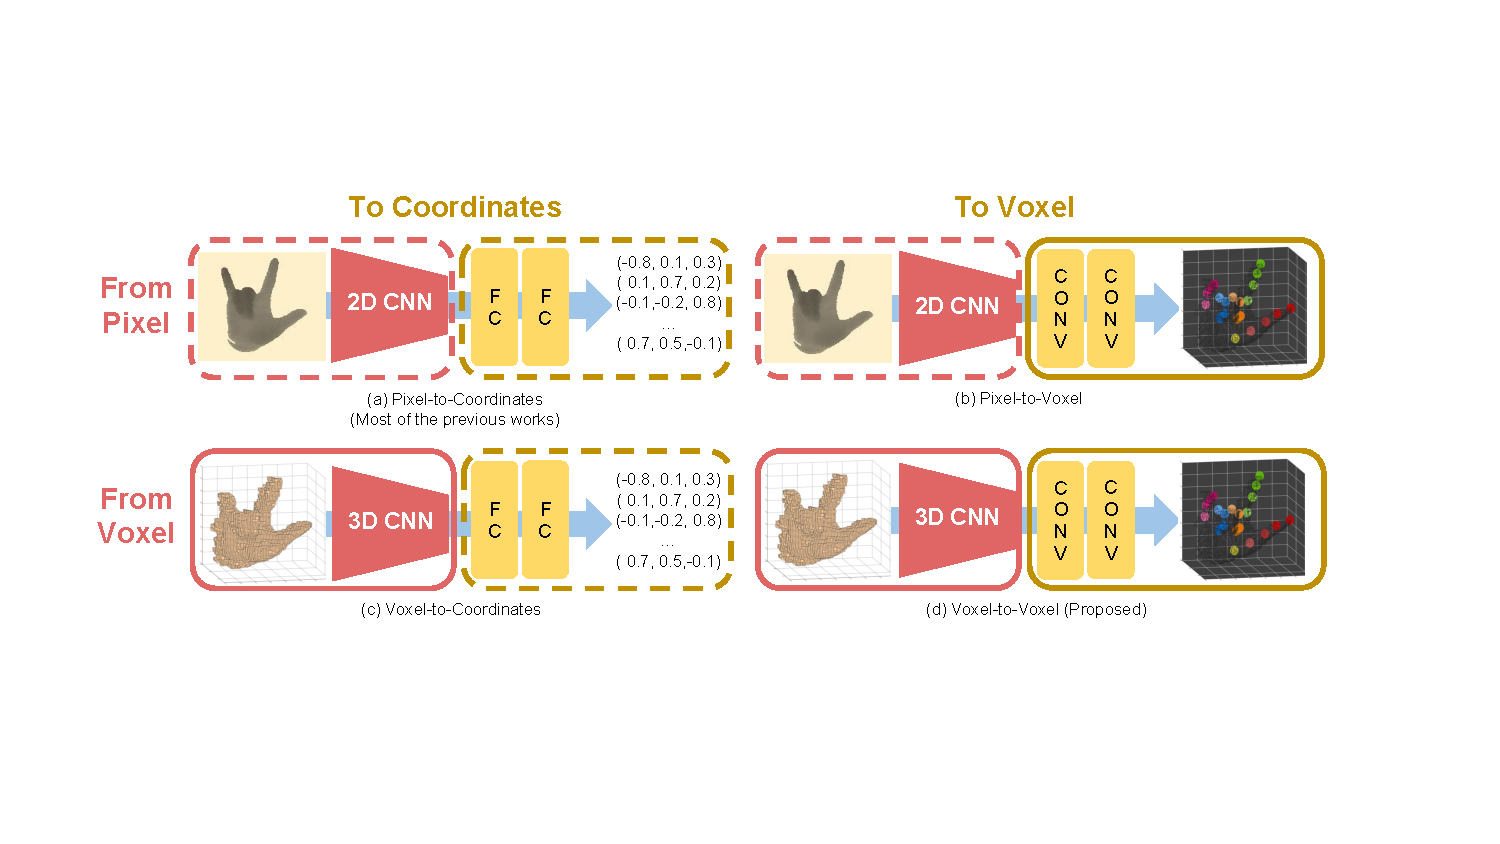
\includegraphics[width=1.0\linewidth]{comparison_io_type.pdf}
\end{center}
\vspace*{-5mm}
   \caption{Various combinations of inputs and outputs for 3D pose estimation from a single depth image. Most of the previous works take a 2D depth image as input and estimate the 3D coordinates of keypoints as in (a). In contrast, the proposed system takes a 3D voxelized grid and estimates the per-voxel likelihood of each keypoint as in (d). Note that (b) and (d) are solely composed of the convolutional layers that become the fully convolutional architecture.}
\label{fig:comparison_io_type}
\end{figure*}

\section{Related works}

{\bf Depth-based 3D hand pose estimation.} 
Hand pose estimation methods can be categorized into generative, discriminative, and hybrid methods. Generative methods assume a pre-defined hand model and fit it to the input depth image by minimizing hand-crafted cost functions ~\cite{sharp2015accurate, tang2015opening}. Particle swam optimization (PSO)~\cite{sharp2015accurate}, iterative closest point (ICP)~\cite{tagliasacchi2015robust}, and their combination~\cite{qian2014realtime} are the common algorithms used to obtain optimal hand pose results.

Discriminative methods directly localize hand joints from an input depth map. Random forest-based methods~\cite{keskin2012hand,tang2013real,tang2014latent,liang2014parsing,sun2015cascaded,tang2015opening,wan2016hand} provide fast and accurate performance. However, they utilize hand-crafted features and are overcome by recent CNN-based approaches ~\cite{tompson2014real,oberweger2015hands,ge2016robust,sinha2016deephand,bouchacourt2016disco,yang2016hand,deng2017hand3d,ge20173d,guo2017ren,guo2017towards,chen2017pose,madadi2017end,fourure2017multi,xu2017lie,Choi_2017_ICCV,Oberweger_2017_ICCV_Workshops} that can learn useful features by themselves. Tompson \etal~\cite{tompson2014real} firstly utilized CNN to localize hand keypoints by estimating 2D heatmaps for each hand joint. Ge \etal~\cite{ge2016robust} extended this method by exploiting multi-view CNN to estimate 2D heatmaps for each view. Ge \etal~\cite{ge20173d} transformed the 2D input depth map to the 3D form and estimated 3D coordinates directly via 3D CNN. Guo \etal~\cite{guo2017ren,guo2017towards} proposed a region ensemble network to accurately estimate the 3D coordinates of hand keypoints and Chen \etal~\cite{chen2017pose} improved this network by iteratively refining the estimated pose. Oberweger \etal~\cite{Oberweger_2017_ICCV_Workshops} improved their preceding work~\cite{oberweger2015hands} by utilizing recent network architecture, data augmentation, and better initial hand localization.

Hybrid methods are proposed to combine the generative and discriminative approach. Oberweger \etal~\cite{oberweger2015training} trained discriminative and generative CNNs by a feedback loop. Zhou \etal~\cite{zhou2016model} pre-defined a hand model and estimated the parameter of the model instead of regressing 3D coordinates directly. Ye \etal~\cite{ye2016spatial} used spatial attention mechanism and hierarchical PSO. Wan \etal~\cite{Wan_2017_CVPR} used two deep generative models with a shared latent space and trained discriminator to estimate the posterior of the latent pose.


{\bf Depth-based 3D human pose estimation.} 
Depth-based 3D human pose estimation methods also rely on generative and discriminative models. The generative models estimate the pose by finding the correspondences between the pre-defined body model and the input 3D point cloud. The ICP algorithm is commonly used for 3D body tracking~\cite{ganapathi2012real,grest2005nonlinear,knoop2006sensor,helten2013personalization}. Another method such as template fitting with Gaussian mixture models ~\cite{ye2014real} was also proposed. By contrast, the discriminative models do not require body templates and they directly estimate the positions of body joints. Conventional discriminative methods are mostly based on random forests. Shotton \etal~\cite{shotton2013real} classified each pixel into one of the body parts, while Girchick \etal~\cite{girshick2011efficient} and Jung \etal~\cite{jung2016sequential} directly regressed the coordinates of body joints. Jung \etal~\cite{yub2015random} used a random tree walk algorithm (RTW), which reduced the running time significantly. Recently, Haque \etal~\cite{haque2016towards} proposed the viewpoint-invariant pose estimation method using CNN and multiple rounds of a recurrent neural network. Their model learns viewpoint-invariant features, which makes the model robust to viewpoint variations.

\begin{figure*}
\begin{center}
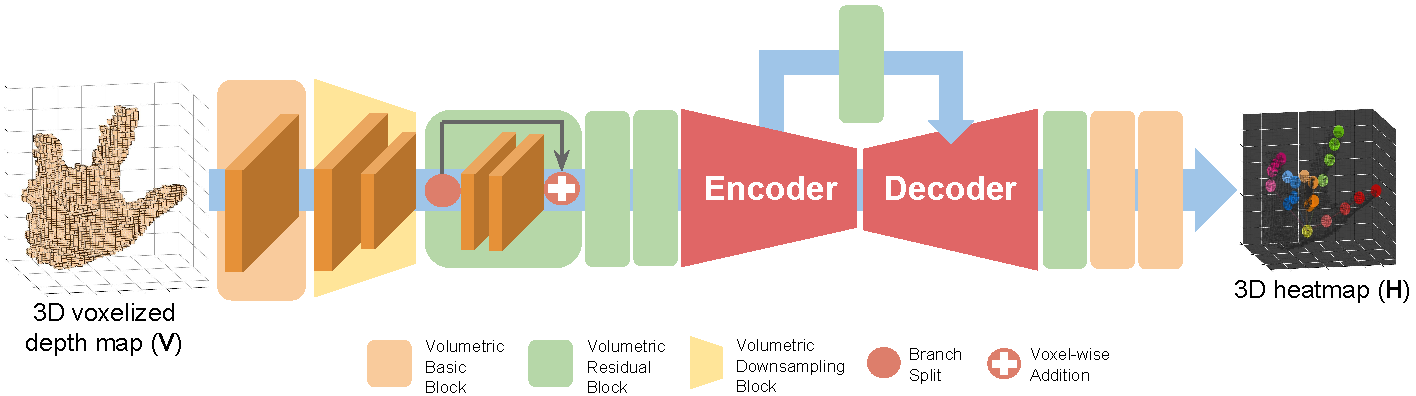
\includegraphics[width=1.0\linewidth]{model_architecture.pdf}
\end{center}
\vspace*{-5mm}
   \caption{Overall architecture of the V2V-PoseNet. V2V-PoseNet takes voxelized input and estimates the per-voxel likelihood for each keypoint through encoder and decoder. To simplify the figure, we plotted each feature map without Z-axis and combined the 3D heatmaps of all keypoints in a single volume. Each color in the 3D heatmap indicates keypoints in the same finger.}
\vspace*{-3mm}
\label{fig:model_architecture}
\end{figure*}

{\bf Volumetric representation using depth information.}
Wu \etal~\cite{wu20153d} introduced the volumetric representation of a depth image and surpassed the existing hand-crafted descriptor-based methods in 3D shape classification and retrieval. They represented each voxel as a binary random variable and used a convolutional deep belief network to learn the probability distribution for each voxel. Several recent works~\cite{maturana2015voxnet,song2016deep} also represented 3D input data as a volumetric form for 3D object classification and detection. Our work follows the strategy from ~\cite{maturana2015voxnet}, wherein several types of volumetric representation (i.e., occupancy grid models) were proposed to fully utilize the rich source of 3D information and efficiently deal with large amounts of point cloud data. Their proposed CNN architecture and occupancy grids outperform those of Wu \etal~\cite{wu20153d}.

{\bf Input and output representation in 3D pose estimation.}
Most of the existing methods for 3D pose estimation from a single depth map~\cite{oberweger2015hands,oberweger2015training,bouchacourt2016disco,Wan_2017_CVPR,guo2017ren,guo2017towards,Oberweger_2017_ICCV_Workshops,chen2017pose,madadi2017end,fourure2017multi,haque2016towards} are based on the model in Figure~\ref{fig:comparison_io_type}(a) that takes a 2D depth image and directly regresses 3D coordinates. Recently, Ge \etal~\cite{ge20173d} and Deng \etal~\cite{deng2017hand3d} converted a 2D depth image to a truncated signed distance function-based 3D volumetric form and directly regressed 3D coordinates as shown in Figure~\ref{fig:comparison_io_type}(c). In 3D human pose estimation from a RGB image, Pavlakos \etal~\cite{pavlakos2016coarse} estimated the per-voxel likelihood for each body keypoint via 2D CNN as in the Figure~\ref{fig:comparison_io_type}(b). To estimate the per-voxel likelihood from an RGB image, they treated the discretized depth value as a channel of the feature map, which resulted in different kernels for each depth value. In contrast to all the above approaches, our proposed system estimates the per-voxel likelihood of each keypoint via the 3D fully convolutional network from the voxelized input as in Figure~\ref{fig:comparison_io_type}(d). To the best of our knowledge, our network is the first model to generate voxelized output from voxelized input using 3D CNN for 3D pose estimation.









\section{Overview of the proposed model}

The goal of our model is to estimate the 3D coordinates of all keypoints. First, we convert 2D depth images to 3D volumetric forms by reprojecting the points in the 3D space and discretizing the continuous space. After voxelizing the 2D depth image, the V2V-PoseNet takes the 3D voxelized data as an input and estimates the per-voxel likelihood for each keypoint. The position of the highest likelihood response for each keypoint is identified and warped to the real world coordinate, which becomes the final result of our model. Figure~\ref{fig:model_architecture} shows the overall architecture of the proposed V2V-PoseNet. We now describe the target object localization refinement strategy, the process of generating the input of the proposed model, V2V-PoseNet, and some related issues of the proposed approach in the following sections.

\begin{figure}[t]
\begin{center}
   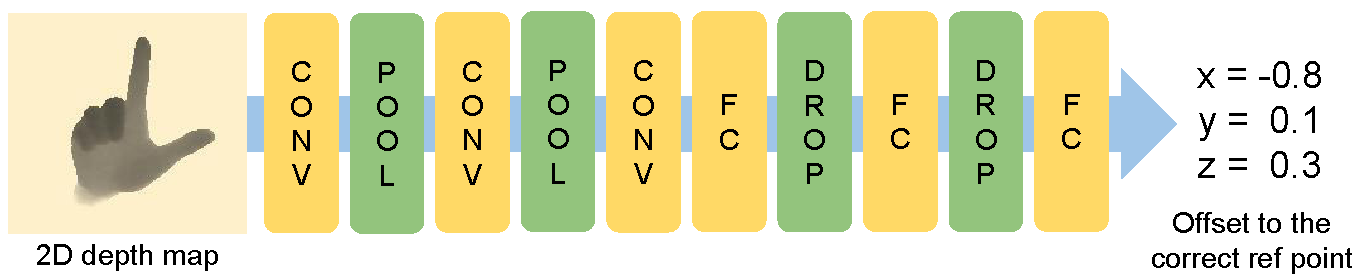
\includegraphics[width=1.0\linewidth]{ref_refine_net.pdf}
\end{center}
\vspace*{-5mm}
   \caption{Reference point refining network. This network takes cropped depth image and outputs the 3D offset from the current reference point to the center of ground-truth joint locations.}
\vspace*{-3mm}
\label{fig:ref_refine_net}
\end{figure}



\section{Refining target object localization}
\label{refineRefPoint_Section}

To localize keypoints, such as hand or human body joints, a cubic box that contains the hand or human body in 3D space is a prerequisite. This cubic box is usually placed around the reference point, which is obtained using ground-truth joint position~\cite{oberweger2015hands,oberweger2015training,zhou2016model} or the center-of-mass after simple depth thresholding around the hand region~\cite{guo2017ren,guo2017towards,chen2017pose}. However, utilizing the ground-truth joint position is infeasible in real-world applications. Also, in general, using the center-of-mass calculated by simple depth thresholding does not guarantee that the object is correctly contained in the acquired cubic box due to the error in the center-of-mass calculations in cluttered scenes. For example, if other objects are near the target object, then the simple depth thresholding method cannot properly filter the other objects because it applies the same threshold value to all input data. Hence, the computed center-of-mass becomes erroneous, which results in a cubic box that contains only some part of the target object. To overcome these limitations, we train a simple 2D CNN following Oberweger \etal~\cite{Oberweger_2017_ICCV_Workshops} to obtain an accurate reference point as shown in Figure~\ref{fig:ref_refine_net}. This network takes a depth image, whose reference point is calculated by the simple depth thresholding around the hand region, and outputs 3D offset from the calculated reference point to the center of ground-truth joint locations. The refined reference point can be obtained by adding the output offset value of the network to the calculated reference point.

\section{Generating input of the proposed system}

To create the input of the proposed system, the 2D depth map should be converted to voxelized form. To voxelize the 2D depth map, we first reproject each pixel of the depth map to the 3D space. After reprojecting all depth pixels, the 3D space is discretized based on the pre-defined voxel size. Then, the target object is extracted by drawing the cubic box around the reference point obtained in Section~\ref{refineRefPoint_Section}. We set the voxel value of the network's input $V(i,j,k)$ as 1 if the voxel is occupied by any depth point and 0 otherwise.

\section{V2V-PoseNet}
\label{V2V-PoseNet_Section}

\subsection{Building block design}
We use four kinds of building blocks in designing the V2V-PoseNet. The first one is the \emph{volumetric basic block} that consists of a volumetric convolution, volumetric batch normalization~\cite{ioffe2015batch}, and the activation function (i.e., ReLU). This block is located in the first and last parts of the network. The second one is the \emph{volumetric residual block} extended from the 2D residual block of option B in ~\cite{he2016deep}. The third one is the \emph{volumetric downsampling block} that is identical to a volumetric max pooling layer. The last one is the \emph{volumetric upsampling block}, which consists of a volumetric deconvolution layer, volumetric batch normalization layer, and the activation function (i.e., ReLU). Adding the batch normalization layer and the activation function to the deconvolution layer helps to ease the learning procedure. The kernel size of the residual blocks is 3$\times$3$\times$3 and that of the downsampling and upsampling layers is 2$\times$2$\times$2 with stride 2.


\begin{figure}[t]
\begin{center}
   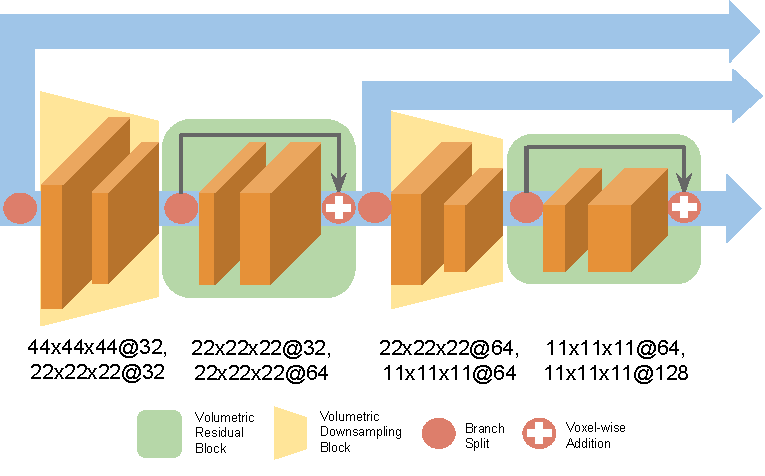
\includegraphics[width=1.0\linewidth]{encoder.pdf}
\end{center}
\vspace*{-5mm}
   \caption{Encoder of the V2V-PoseNet. The numbers below each block indicate the spatial size and number of channels of each feature map. We plotted each feature map without Z-axis to simplify the figure.}
\vspace*{-4mm}
\label{fig:encoder}
\end{figure}


\subsection{Network design}
The V2V-PoseNet performs voxel-to-voxel prediction. Thus, it is based on the 3D CNN architecture that treats the Z-axis as an additional spatial axis so that the kernel shape is $w$$\times$$h$$\times$$d$. Our network architecture is based on the hourglass model~\cite{newell2016stacked}, which was slightly modified for more accurate estimation. As the Figure~\ref{fig:model_architecture} shows, the network starts from the 7$\times$7$\times$7 volumetric basic block and the volumetric downsampling block. After downsampling the feature map, three consecutive residual blocks extract useful local features. The output of the residual blocks goes through the encoder and decoder described in Figures~\ref{fig:encoder} and ~\ref{fig:decoder}, respectively.

In the encoder, the volumetric downsampling block reduces the spatial size of the feature map while the volumetric residual bock increases the number of channels. It is empirically confirmed that this increase in the number of channels helps improve the performance in our experiments. On the other hand, in the decoder, the volumetric upsampling block enlarges the spatial size of the feature map. When upsampling, the network decreases the number of channels to compress the extracted features. The enlargement of the volumetric size in the decoder helps the network to densely localize keypoints because it reduces the stride between voxels in the feature map. The encoder and decoder are connected with the voxel-wise addition for each scale so that the decoder can upsample the feature map more stably. After passing the input through the encoder and decoder, the network predicts the per-voxel likelihood for each keypoint through two 1$\times$1$\times$1 volumetric basic blocks and one 1$\times$1$\times$1 volumetric convolutional layer.


\begin{figure}[t]
\begin{center}
   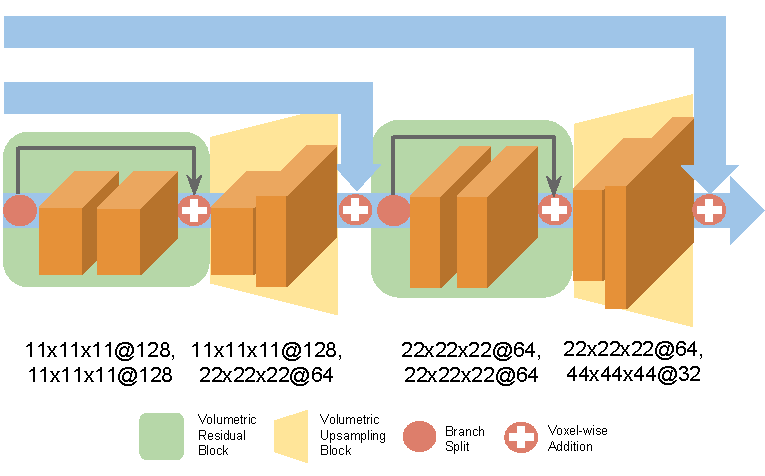
\includegraphics[width=1.0\linewidth]{decoder.pdf}
\end{center}
\vspace*{-5mm}
   \caption{Decoder of the V2V-PoseNet. The numbers below each block indicate the spatial size and number of channels of each feature map. We plotted feature map without Z-axis to simplify the figure.}
\vspace*{-4mm}
\label{fig:decoder}
\end{figure}



\subsection{Network training}
To supervise the per-voxel likelihood for each keypoint, we generate 3D heatmap, wherein the mean of Gaussian peak is positioned at the ground-truth joint location as follows: 

\begin{equation}
H_{\mathrm{n}}^*(i,j,k) = \exp\left(-\frac{(i-i_{\mathrm{n}})^2+(j-j_{\mathrm{n}})^2+(k-k_{\mathrm{n}})^2}{2\sigma^2}\right),
\end{equation}
where $H_{n}^{*}$ is the ground-truth 3D heatmap of $n$th keypoint, ($i_n$,$j_n$,$k_n$) is the ground-truth voxel coordinate of $n$th keypoint, and $\sigma$ = 1.7 is the standard deviation of the Gaussian peak.

Also, we adopt the mean square error as a loss function $L$ as follows:

\begin{equation}
L = \sum_{n=1}^{N} \sum_{i,j,k} \|H_{\mathrm{n}}^*(i,j,k)-H_{\mathrm{n}}(i,j,k)\|^2,
\end{equation}
where $H_{n}^{*}$ and $H_{n}$ are the ground-truth and estimated heatmaps for $n$th keypoint, respectively, and $N$ denotes the number of keypoints.




\section{Implementation details}
The proposed V2V-PoseNet is trained in an end-to-end manner from scratch. All weights are initialized from the zero-mean Gaussian distribution with $\sigma$ = 0.001. Gradient vectors are calculated from the loss function and the weights are updated by the RMSProp~\cite{tieleman2012lecture} with a mini-batch size of 8. The learning rate is set to 2.5$\times$$10^{-4}$. The size of the input to the proposed system is 88$\times$88$\times$88. We perform data augmentation including rotation ([-40, 40] degrees in XY space), scaling ([0.8, 1.2] in 3D space), and translation ([-8, 8] voxels in 3D space). Our model is implemented by Torch7~\cite{collobert2011torch7} and the NVIDIA Titan X GPU is used for training and testing. We trained our model for 10 epochs.


\section{Experiments}
\vspace{-0.05in}

In this section, we conduct a series of experiments to evaluate our model. 
To explore whether the model learns to perform the spatial inference necessary for answering visual questions that explicitly require spatial reasoning, we design a set of experiments using synthetic visual question/answer data in Sec.~\ref{sec:synthetic1}. The experimental results of our model in standard datasets (DAQUAR~\cite{DBLP:journals/corr/MalinowskiF14} and VQA~\cite{DBLP:journals/corr/AntolALMBZP15} datasets) are reported in Sec.~\ref{sec:expstandard}.

%%%%%%%%%%%%%%%%%%%%%%%%%%%%%%%%%%%%%%%%%%%%%%%%%%%%%%%%%%%%%%%%%%%%%%%%%%%%%%%%%%%%%%%%%%%%%%%%%%%
\subsection{Exploring Attention on Synthetic Data}\label{sec:synthetic1}
%Several public datasets are available, however, 
The questions in the public VQA datasets are quite varied and difficult and often require common sense knowledge to answer (e.g., ``Does this man have 20/20 vision?'' about a person wearing glasses). Furthermore, past work~\cite{malinowski2015ask,DBLP:journals/corr/RenKZ15} showed that the question text alone (no image) is a very strong predictor of the answer.
Therefore, before evaluating on standard datasets, we would first like to
understand how the proposed model uses spatial attention to answer simple visual questions where the answer cannot be predicted from question alone. 
Our visualization demonstrates that the attention mechanism does learn to attend to objects and gather evidence via certain inference rules. 

%%%%%%%%%%% figure
\begin{figure*}[!t]
  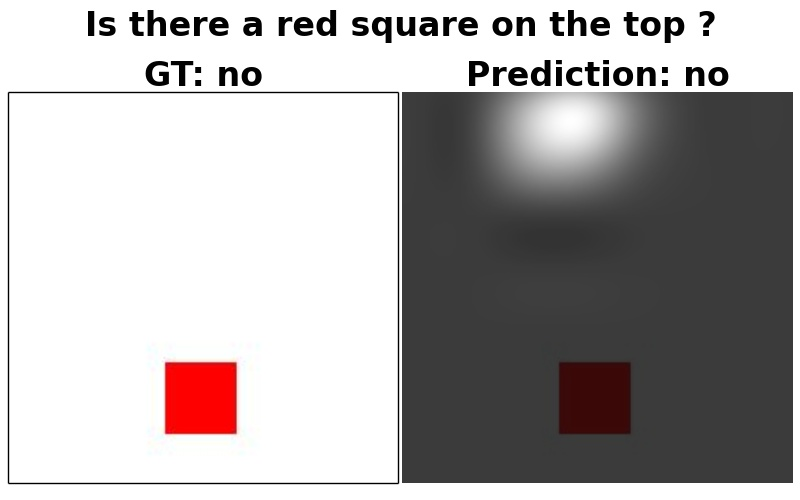
\includegraphics[width=0.242\textwidth]{figures/rule1_im_30075_219_top.JPEG}
  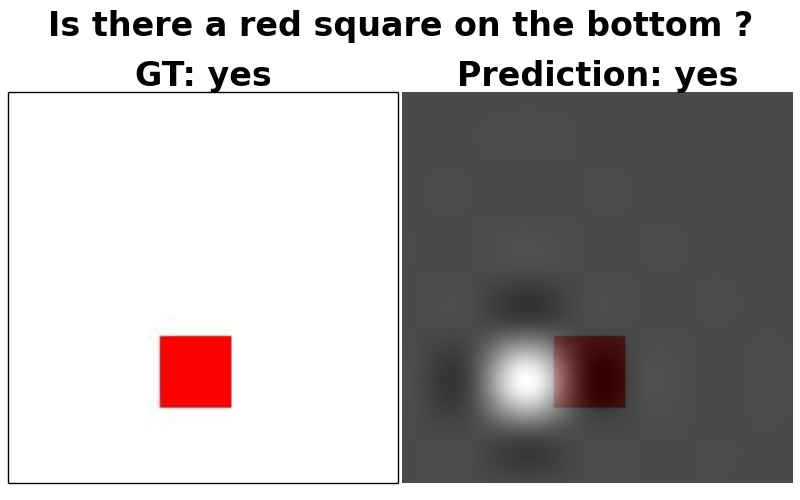
\includegraphics[width=0.242\textwidth]{figures/rule1_im_31186_4441_bottom.JPEG}
  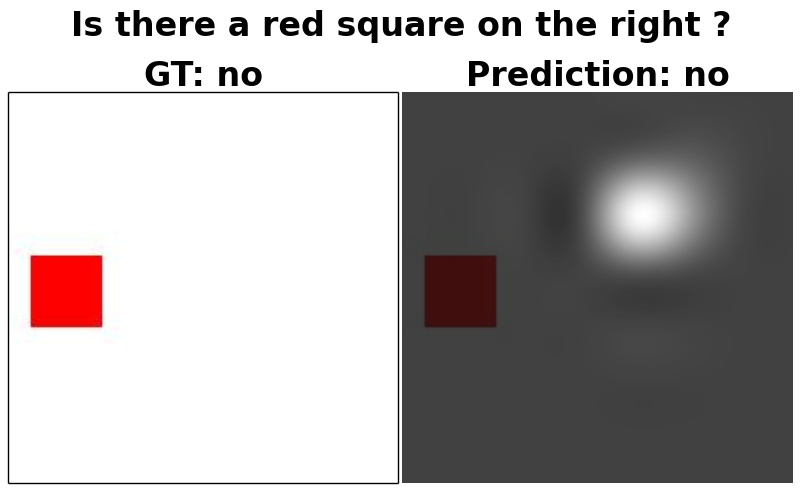
\includegraphics[width=0.242\textwidth]{figures/rule1_im_31189_690_right.JPEG}
  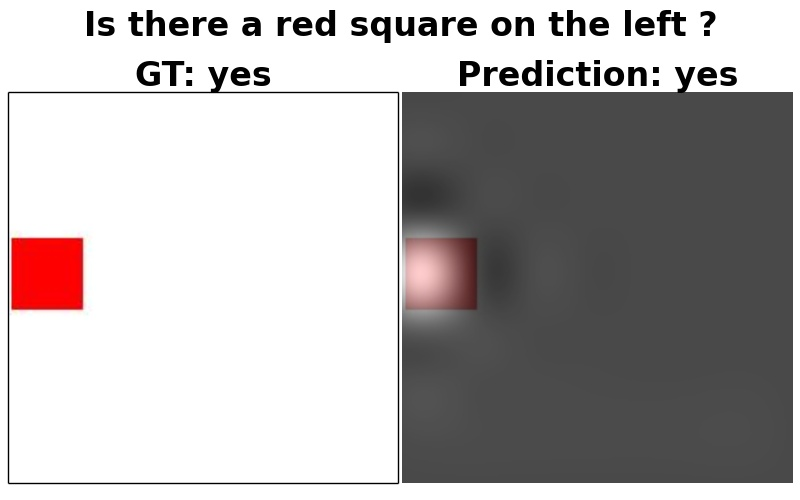
\includegraphics[width=0.242\textwidth]{figures/rule1_im_31200_4217_left.JPEG}\\
  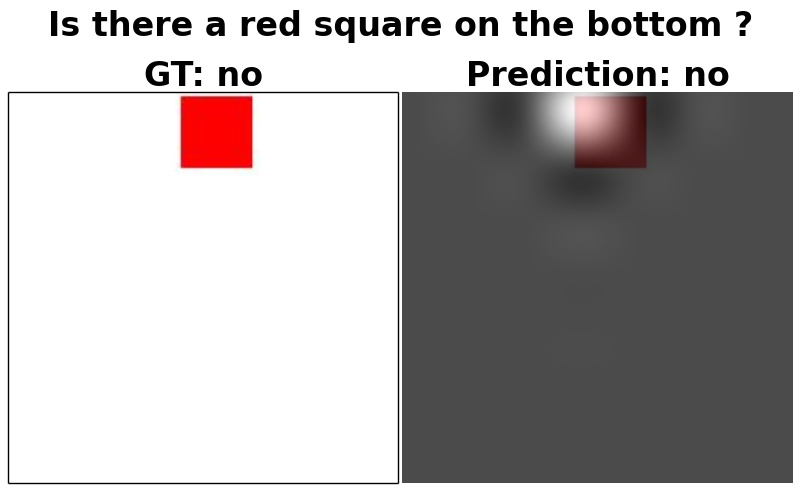
\includegraphics[width=0.242\textwidth]{figures/rule2_im_30004_3495_bottom.JPEG}
  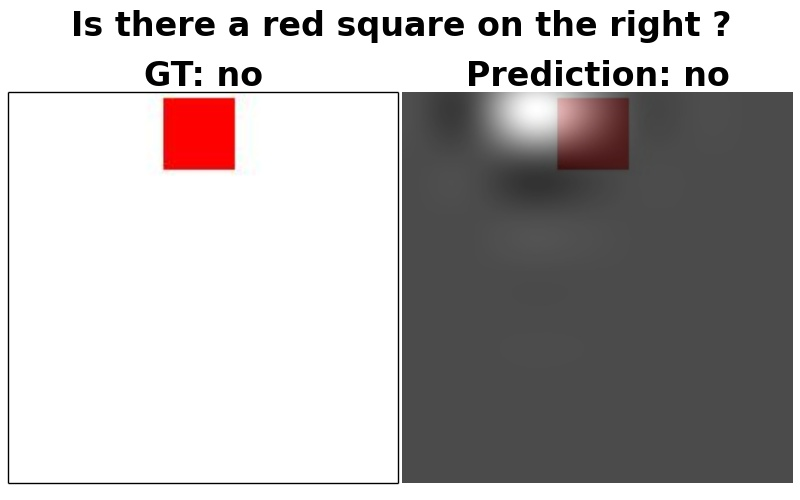
\includegraphics[width=0.242\textwidth]{figures/rule2_im_30036_3165_right.JPEG}
  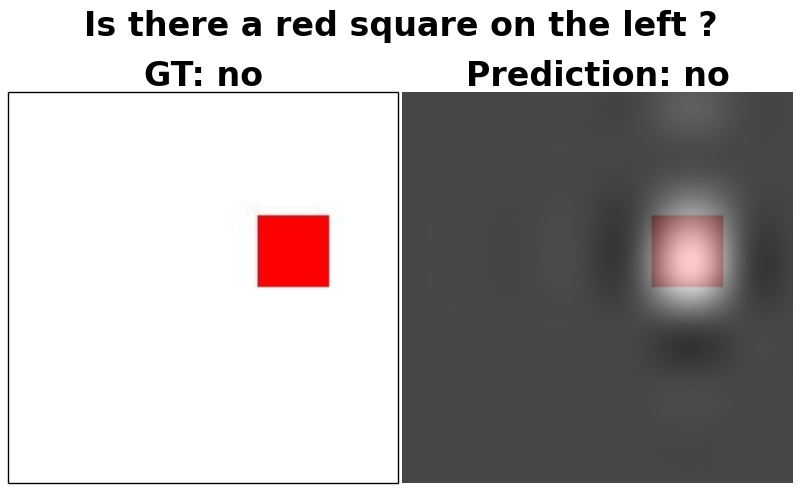
\includegraphics[width=0.242\textwidth]{figures/rule2_im_31185_2199_left.JPEG}
  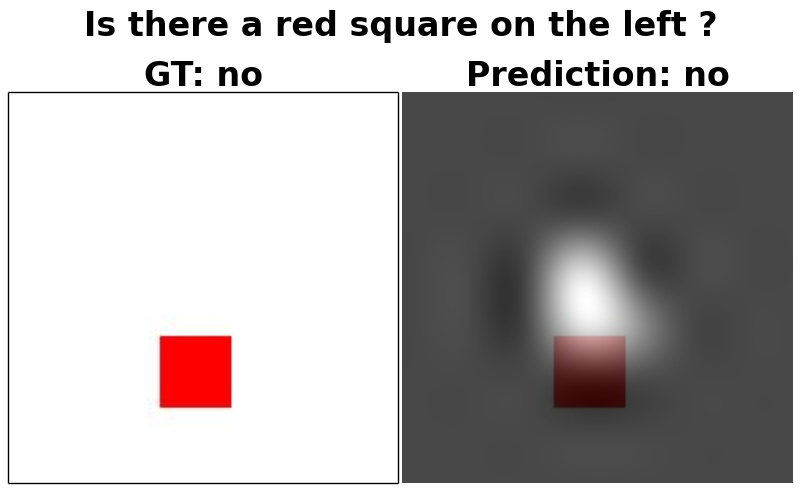
\includegraphics[width=0.242\textwidth]{figures/rule2_im_31186_1310_left.JPEG}
%\includegraphics[width=\textwidth]{figures/onehop_twohop.png}
\vspace{-0.1in}
\caption{\textbf{Absolute position experiment:} for each image and question pair, we show the original image (left) and the attention weights $W_{att}$ (right). 
The attention follows the following rules. The first rule (top row) looks at the position specified in question (top$\mid$bottom$\mid$right$\mid$left), if it contains a square, answer ``yes''; otherwise answer ``no''.
The second rule (bottom row) looks at the region where there is a square, and answers ``yes'' if the question contains that position and ``no'' for the other three positions.}\label{fig:red_square}
\vspace{-0.1in}
\end{figure*}


%%%%%%%%%%%%%%%%%%%%%%%%%%%%%%%%%%%%%%%%%%%%%%%%%%%%%%%%%%%%%%%%%%%%%%%%%%%%%%%%%%%%%%%%%%%%%%%%%%%
\vspace{-0.1in}
\subsubsection{Absolute Position Recognition}\label{sec:absolute}
We investigate whether the model has the ability to recognize the absolute location of the object in the image. We explore this by designing a simple task where an object (a red square) appears in some region of a white-background image, and the question is ``Is there a red square on the [top$\mid$bottom$\mid$left$\mid$right]?'' For each image, we randomly place the square in one of the four regions, and generate the four questions above, together with three ``no'' answers and one ``yes'' answer. The generated data is split into training and testing sets. 

Due to the simplicity of this synthetic dataset, the SMem-VQA one-hop model achieves 100\% test accuracy. However, the baseline model (iBOWIMG)~\cite{zhou2015simple} cannot infer the answer and only obtains accuracy of around 75\%, which is the prior probability of the answer ``no'' in the training set. The SMem-VQA one-hop model is equivalent to the iBOWIMG model if the attention weights in our one-hop model are set equally for each location, since the iBOWIMG model uses the mean pool of the convolutional feature ($inception\_5b/output$) in GoogLeNet that we use in SMem-VQA model. 
We check the visualization of the attention weights and find that the relationship between the high attention position and the answer can be expressed by logical expressions.
We show the attention weights of several typical examples in Fig.~\ref{fig:red_square} which reflect two logic rules:
1)~Look at the position specified in question (top$\mid$bottom$\mid$right$\mid$left), if it contains a square, then answer ``yes''; if it does not contain a square, then answer ``no''.
2)~Look at the region where there is a square, then answer ``yes'' for the question about that position and ``no'' for the questions about the other three positions.

In the iBOWIMG model, the mean-pooled GoogLeNet visual features lose spatial information and thus cannot distinguish images with a square in different positions. On the contrary, our SMem-VQA model can pay high attention to different regions according to the question, and generate an answer based on the selected region, using some learned inference rules.
This experiment demonstrates that the attention mechanism in our model is able to make absolute spatial location inference based on the spatial attention. 


%%%%%%%%%%% figure
\begin{figure*}[t]
  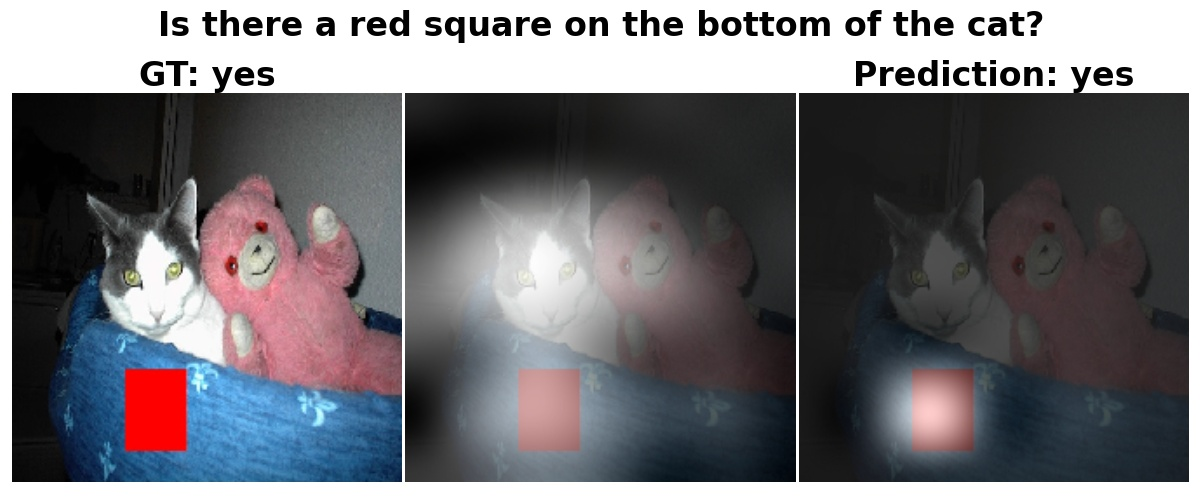
\includegraphics[width=0.325\textwidth]{figures/bottom_COCO_val2014_000000167602_bottom.jpg}
  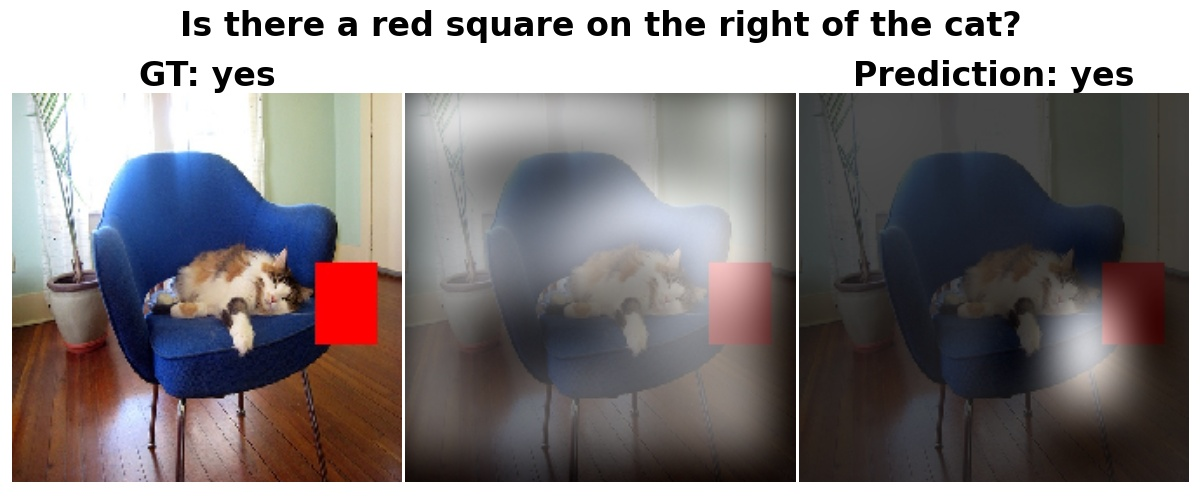
\includegraphics[width=0.325\textwidth]{figures/right_COCO_val2014_0000002988_right.jpg}
  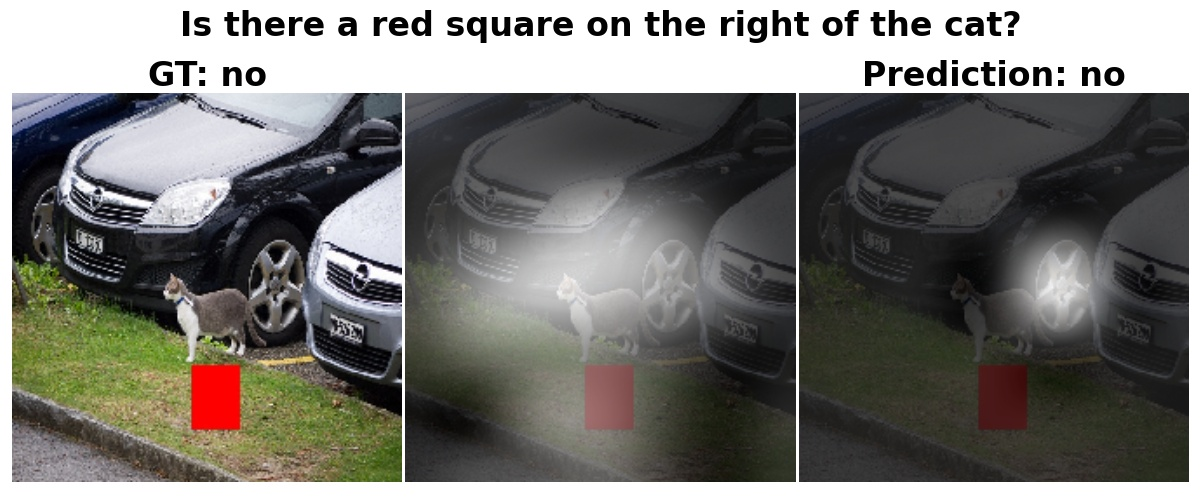
\includegraphics[width=0.325\textwidth]{figures/right_COCO_val2014_000000172330_bottom.jpg}\\
  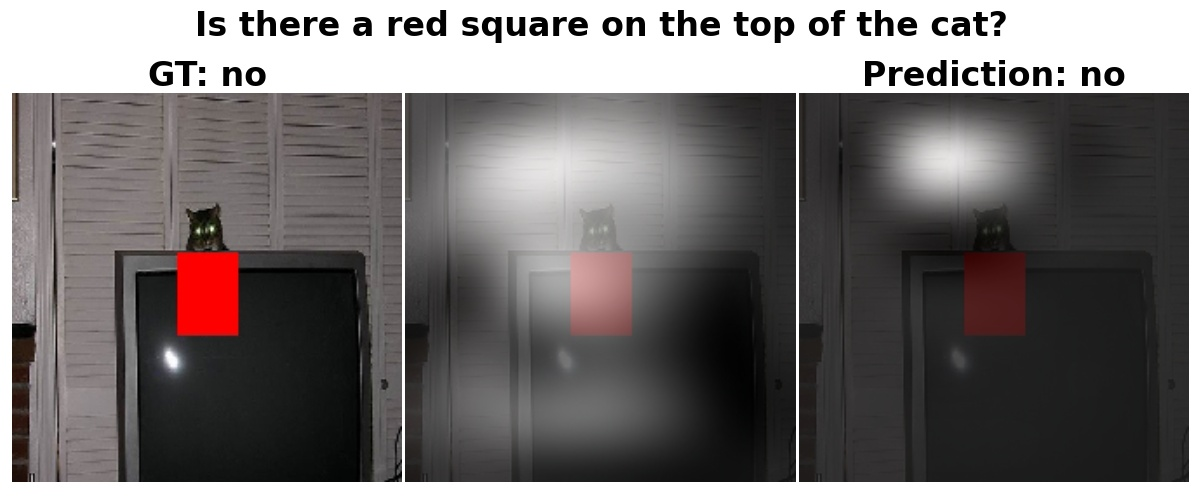
\includegraphics[width=0.325\textwidth]{figures/top_COCO_val2014_00000010694_bottom}
  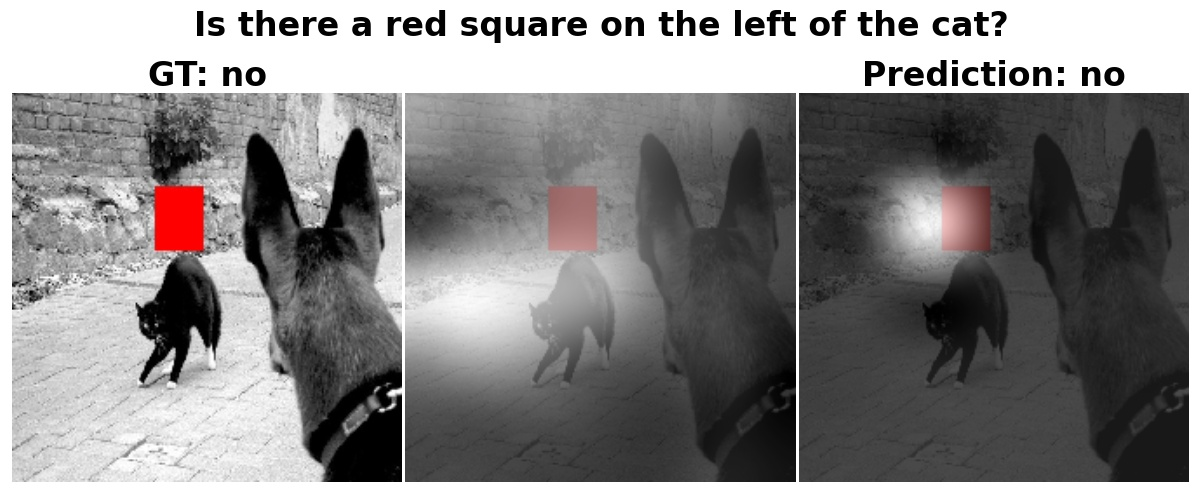
\includegraphics[width=0.325\textwidth]{figures/left_COCO_val2014_000000201918_top.jpg}
  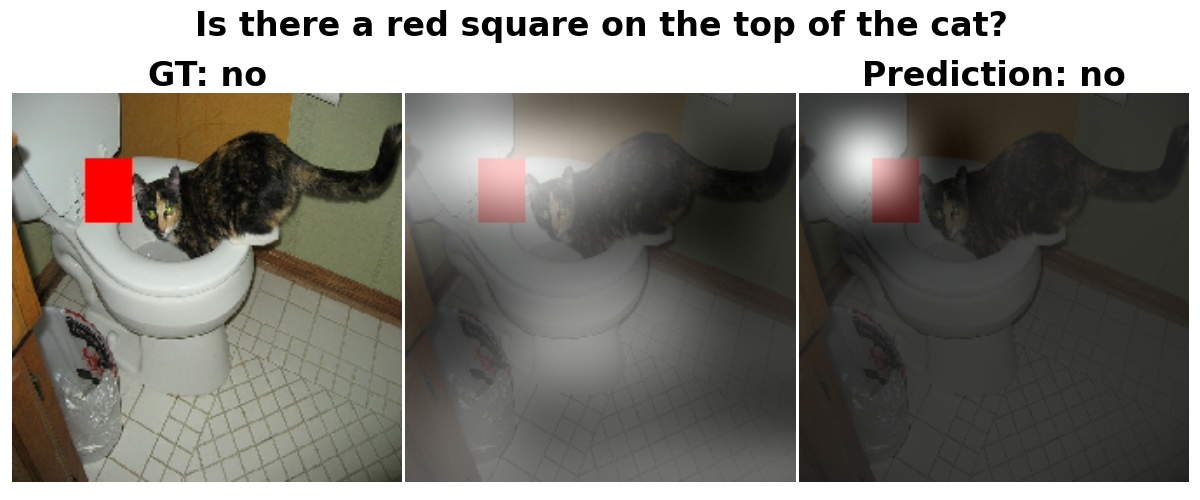
\includegraphics[width=0.325\textwidth]{figures/top_COCO_val2014_000000218924_left.jpg}
\vspace{-0.05in}
\caption{\textbf{Relative position experiment:}
for each image and question pair, we show the original image (left), the evidence embedding $W_E$ of the convolutional layer (middle) and the attention weights $W_{att}$ (right). The evidence embedding $W_E$ has high activations on both cat and red square. 
The attention weights follow similar inference rules as in Fig.~\ref{fig:red_square}, with the difference that the attention position is around the cat.
%Rule#1: (top row) look at the specified position (top/bottom/right/left), if it contains a square, answer "yes"; otherwise answer "no".
%Rule#2: (bottom row) look at the region where there is a square, answer "yes" if the question contains that position and "no" if it contains one of the other three positions.
}\label{fig:cat_square}
\vspace{-0.2in}
\end{figure*}


%%%%%%%%%%%%%%%%%%%%%%%%%%%%%%%%%%%%%%%%%%%%%%%%%%%%%%%%%%%%%%%%%%%%%%%%%%%%%%%%%%%%%%%%%%%%%%%%%%%
\vspace{-0.1in}
\subsubsection{Relative Position Recognition}
In order to check whether the model has the ability to infer the  position of one object \textit{relative} to another object,
we collect all the cat images from the MS COCO Detection dataset~\cite{lin2014microsoft}, and add a red square on the [top$\mid$bottom$\mid$left$\mid$right] of the bounding box of the cat in the images.
For each generated image, we create four questions, ``Is there a red square on the [top$\mid$bottom$\mid$left$\mid$right] of the cat?'' together with three ``no'' answers and one ``yes'' answer. 
We select 2639 training cat images and 1395 testing cat images from MS COCO Detection dataset. 

Our SMem-VQA one-hop model achieves 96\% test accuracy on this synthetic task, while the baseline model (iBOWIMG) accuracy is around 75\%.
We also check that another simple baseline that predicts the answer based on the absolute position of the square in the image gets around 70\% accuracy. 
We visualize the evidence embedding $W_E$ features and the attention weights $W_{att}$ of several typical examples in Fig.~\ref{fig:cat_square}.
The evidence embedding $W_E$ has high activations on the cat and the red square, while the attention weights pay high attention to certain locations around the cat.
We can analyze the attention in the correctly predicted examples using the same rules as in absolute position recognition experiment. 
These rules still work, but the position is relative to the cat object:
1)~Check the specified position relative to the cat, if it finds the square, then answer ``yes'', otherwise ``no''; 2)~Find the square, then answer ``yes'' for the specified position, and answer ``no'' for the other positions around the cat.
We also check the images where our model makes mistakes, and find that the mistakes mainly occur in images with more than one cats. The red square appears near only one of the cats in the image, but our model might make mistakes by focusing on the other cats.
We conclude that our SMem-VQA model can infer the relative spatial position based on the spatial attention around the specified object, which can also be represented by some logical inference rules. 



%%%%%%%%%%%%%%%%%%%%%%%%%%%%%%%%%%%%%%%%%%%%%%%%%%%%%%%%%%%%%%%%%%%%%%%%%%%%%%%%%%%%%%%%%%%%%%%%%%%
%%%%%%%%%%%%%% table
\begin{table}[!t]
\centering
\caption{Accuracy results on the DAQUAR dataset (in percentage).}
\small
 \begin{tabular}{l || c c c} 
 \hline
 ~ & DAQUAR\\ \hline
 Multi-World~\cite{DBLP:journals/corr/MalinowskiF14} & 12.73 \\ %\hline
 Neural-Image-QA~\cite{malinowski2015ask} & 29.27  \\ %\hline
 Question LSTM~\cite{malinowski2015ask} & 32.32 \\ %\hline
 VIS+LSTM~\cite{DBLP:journals/corr/RenKZ15} & 34.41 \\ %\hline
 Question BOW~\cite{DBLP:journals/corr/RenKZ15} & 32.67 \\ %\hline
 IMG+BOW~\cite{DBLP:journals/corr/RenKZ15} & 34.17 \\ \hline
 %2-VIS+BLSTM ~\cite{DBLP:journals/corr/RenKZ15} &  - & 35.78  & -\\ \hline \hline
 %Question One-Hop & 53.37 & 36.03 & - \\ %\hline   
 SMem-VQA One-Hop & 36.03 \\ %\hline   
 SMem-VQA Two-Hop & \bf{40.07} \\ \hline 
 %one dimension convolution hierarchy model\cite{ma2015learning} &  - & 0.3933 \cite{ma2015learning} & - \\ \hline
 \end{tabular}
\label{fig:baseline}
\vspace{-0.2in}
\end{table}


\subsection{Experiments on Standard Datasets}\label{sec:expstandard}
%\vspace{-0.08in}
\subsubsection{Results on DAQUAR}
The DAQUAR dataset is a relatively small dataset which builds on the NYU Depth Dataset V2~\cite{Silberman:ECCV12}. We use the reduced DAQUAR dataset~\cite{DBLP:journals/corr/MalinowskiF14}. The evaluation metric for this dataset is 0-1 accuracy. 
The embedding dimension is 512 for our models running on the DAQUAR dataset. 
We use several reported models on DAQUAR as baselines, which are listed below:\\
%\noindent
{$\bullet$} {\bf{Multi-World}}~\cite{DBLP:journals/corr/MalinowskiF14}: an approach based on handcrafted features using a semantic parse of the question and scene analysis of the image combined in a latent-world Bayesian framework.\\ 
{$\bullet$} {\bf{Neural-Image-QA}}~\cite{malinowski2015ask}: uses an LSTM to encode the question and then decode the hidden information into the answer. The image CNN feature vector is shown at each time step of the encoding phase.\\
{$\bullet$} {\bf{Question LSTM}}~\cite{malinowski2015ask}: only shows the question to the LSTM to predict the answer without any image information.\\
{$\bullet$} {\bf{VIS+LSTM}}~\cite{DBLP:journals/corr/RenKZ15}: similar to Neural-Image-QA, but only shows the image features to the LSTM at the first time step, and the question in the remaining time steps to predict the answer.\\
{$\bullet$} {\bf{Question BOW}}~\cite{DBLP:journals/corr/RenKZ15}: only uses the BOW question representation and a single hidden layer neural network to predict the answer, without any image features.\\
{$\bullet$} {\bf{IMG+BOW}}~\cite{DBLP:journals/corr/RenKZ15}: concatenates the BOW question representation with image features, and then uses a single hidden layer neural network to predict the answer. This model is similar to the iBOWIMG baseline model in~\cite{zhou2015simple}.

Results of our SMem-VQA model on the DAQUAR dataset and the baseline model results reported in previous work are shown in Tab.~\ref{fig:baseline}. 
From the DAQUAR result in Tab.~\ref{fig:baseline}, we see that models based on deep features significantly outperform the Multi-World approach based on hand-crafted features. Modeling the question only with either the LSTM model or Question BOW model does equally well in comparison, indicating the the question text contains important prior information for predicting the answer. Also, on this dataset, the VIS+LSTM model achieves better accuracy than Neural-Image-QA model; the former shows the image only at the first timestep of the LSTM, while the latter does so at each timestep. In comparison, both our One-Hop model and Two-Hop spatial attention models outperform the IMG+BOW, as well as the other baseline models.
A major advantage of our model is the ability to visualize the inference process in the deep network. To illustrate this, two attention weights visualization examples in SMem-VQA One-Hop and Two-Hop models on DAQUAR dataset are shown in Fig.~\ref{fig:2hopVQA} (bottom row).



%%%%%%%%%%% figure
\begin{figure*}[t]
%  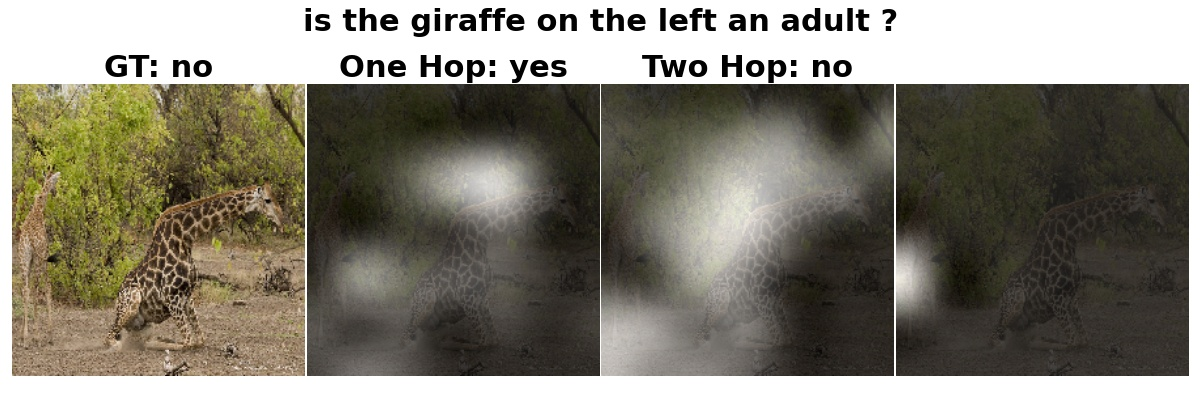
\includegraphics[width=0.5\textwidth]{figures/VQA-DAQUAR_One-Hop_Two-Hop/COCO_val2014_000000014271.jpg}
%  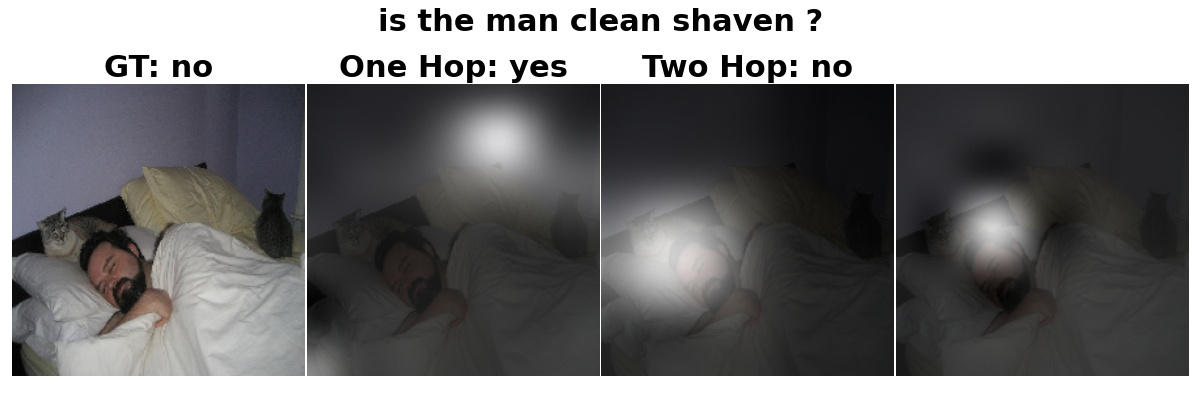
\includegraphics[width=0.5\textwidth]{figures/VQA-DAQUAR_One-Hop_Two-Hop/COCO_val2014_000000012085.jpg}\\
  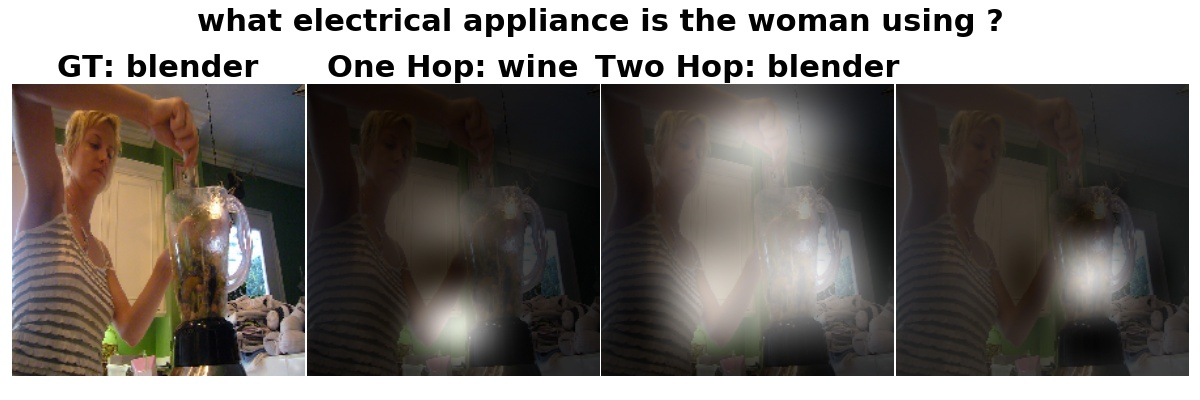
\includegraphics[width=0.5\textwidth]{figures/VQA-DAQUAR_One-Hop_Two-Hop/CO_train2014_000000575060_5750602.jpg}
  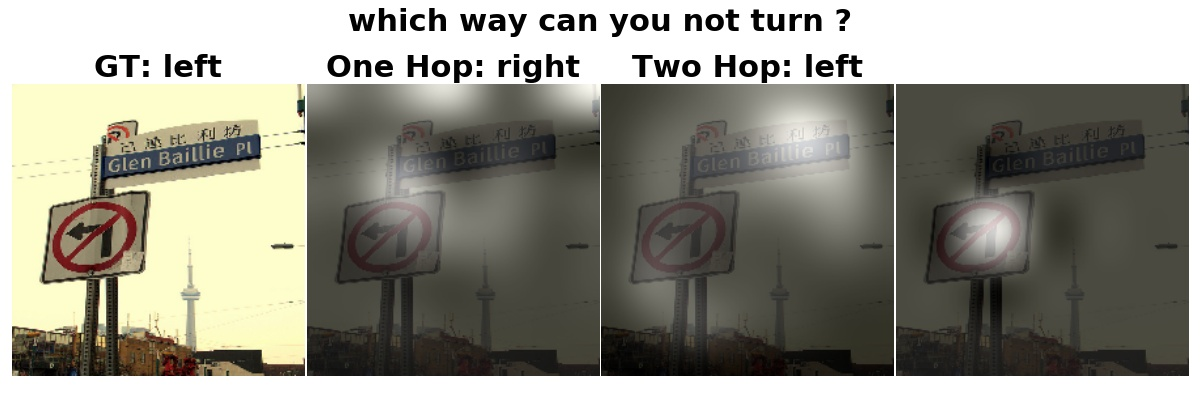
\includegraphics[width=0.5\textwidth]{figures/VQA-DAQUAR_One-Hop_Two-Hop/CO_train2014_000000222383_2223830.jpg}\\
  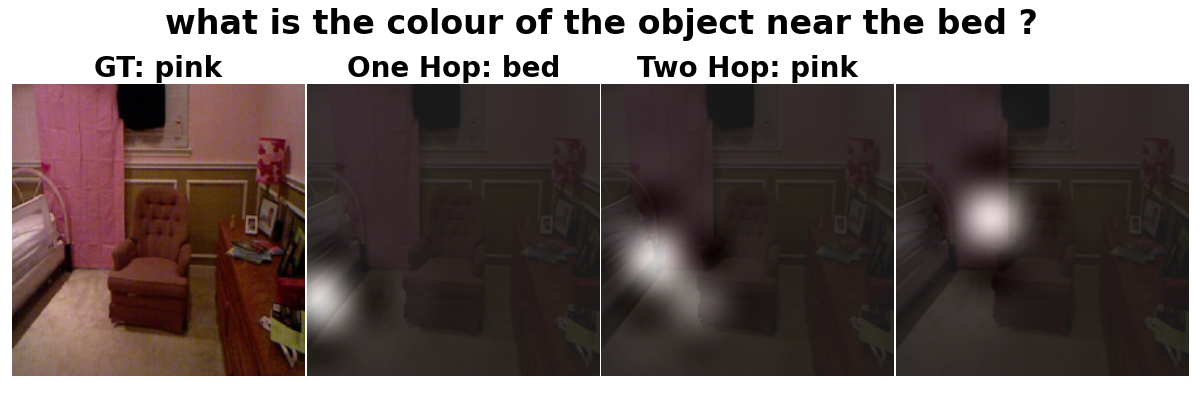
\includegraphics[width=0.5\textwidth]{figures/VQA-DAQUAR_One-Hop_Two-Hop/image1183.png}
  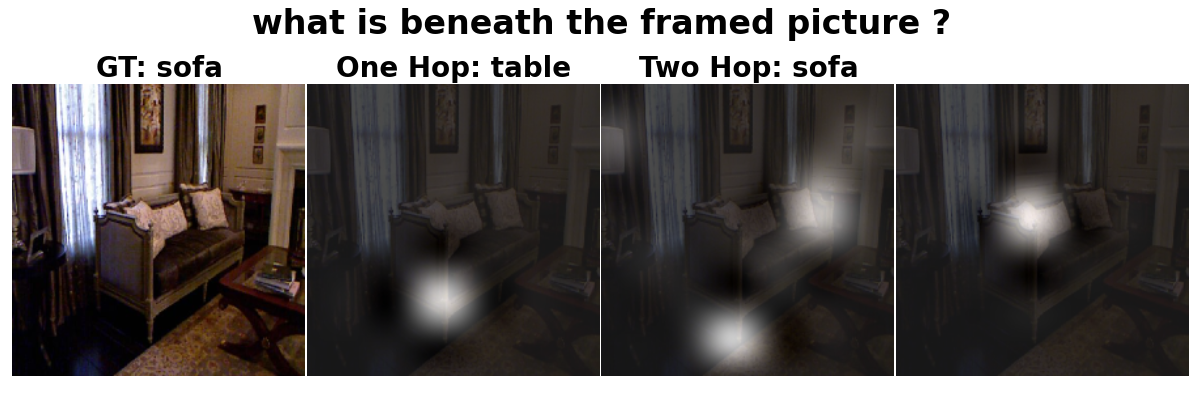
\includegraphics[width=0.5\textwidth]{figures/VQA-DAQUAR_One-Hop_Two-Hop/image1444.png}
\vspace{-0.25in}
\caption{Visualization of the spatial attention weights in the SMem-VQA One-Hop and Two-Hop models on VQA (top row) and DAQUAR (bottom row) datasets. For each image and question pair, we show the original image, the attention weights $W_{att}$ of the One-Hop model, and the two attention weights $W_{att}$ and $W_{att2}$ of the Two-Hop model in order.}\label{fig:2hopVQA}
\vspace{-0.15in}
\end{figure*}
% \vspace{-0.1in}
\subsubsection{Results on VQA}

The VQA dataset is a recent large dataset based on MS COCO~\cite{lin2014microsoft}. We use the full release (V1.0) open-ended dataset, which contains a train set and a val set. Following standard practice, we choose the top 1000 answers in train and val sets as possible prediction answers, and only keep the examples whose answers belong to these 1000 answers as training data. The question vocabulary size is 7477 with the word frequency of at least three.
Because of the larger training size, the embedding dimension is 1000 on the VQA dataset.
We report the test-dev and test-standard results from the VQA evaluation server.
The server evaluation uses the evaluation metric introduced by~\cite{DBLP:journals/corr/AntolALMBZP15}, which gives partial credit to certain synonym answers:
%\begin{equation}
%Acc({\color{red}ans}) = \min\left\{ \frac{\text{\# human that said }{\color{red} ans}}{3},1\right\}
%$Acc({ans}) = \min\left\{ \frac{\text{\# humans that said }{ans}}{3},1\right\}$.
$Acc({ans}) = \min\left\{ (\text{\# humans that said }{ans})/3,1\right\}$.
%\end{equation}


For the attention models, we do not mirror the input image when using the CNN to extract convolutional features, since this might cause confusion about the spatial locations of objects in the input image.
%The input image size for CNN is $224 \times 224$.
The optimization algorithm used is stochastic gradient descent (SGD) with a minibatch of size 50 and momentum of 0.9.
The base learning rate is set to be 0.01 which is halved every six epoches. Regularization, dropout and L2 norm are cross-validated and used. 


%%%%%%%%%%%%%% another candidate table with test-standard
\begin{table}[!t]
\centering
\caption{Test-dev and test-standard results on the Open-Ended VQA dataset (in percentage). Models with ${}^\ast$ use external training data in addition to the VQA dataset.}
\scriptsize
 \begin{tabular}{l || c c c c || c c c c} 
 \hline
 ~ & \multicolumn{4}{c||}{test-dev}  & \multicolumn{4}{c}{test-standard}\\ 
 ~ & \bf{Overall}  & yes/no  & number  & others & \bf{Overall}  & yes/no  & number  & others\\ \hline
 LSTM Q+I~\cite{DBLP:journals/corr/AntolALMBZP15} & 53.74 & 78.94  & 35.24  & 36.42 & 54.06 & -  & -  & -\\ %\hline
 ACK${}^\ast$~\cite{wu2015ask} & 55.72 & 79.23  & 36.13  & 40.08 & 55.98 & 79.05  & 36.10  & 40.61\\ %\hline
 DPPnet${}^\ast$~\cite{noh2015image} & 57.22 & 80.71  & 37.24  & 41.69 & 57.36 & 80.28  & 36.92  & 42.24\\ %\hline
 iBOWIMG~\cite{zhou2015simple} & 55.72 & 76.55  & 35.03  & 42.62 & 55.89 & 76.76  & 34.98  & 42.62\\ \hline 
 SMem-VQA One-Hop & 56.56 & 78.98 & 35.93  & 42.09 & - & -  & -  & -\\ %\hline   
 SMem-VQA Two-Hop & \textbf{57.99} & \textbf{80.87}  & \textbf{37.32}  & \textbf{43.12} & \textbf{58.24} & \textbf{80.8}  & \textbf{37.53}  & \textbf{43.48}\\ \hline 
 \end{tabular}
\label{fig:baseline2}
\vspace{-0.15in}
\end{table}

For the VQA dataset, we use the simple iBOWIMG model in~\cite{zhou2015simple} as one baseline model, which beats most existing VQA models currently on arxiv.org. We also compare to two models in~\cite{wu2015ask}\cite{noh2015image} which have comparable or better results to the iBOWIMG model. These three baseline models as well the best model in VQA dataset paper~\cite{DBLP:journals/corr/AntolALMBZP15} are listed in the following:\\
%\noindent
{$\bullet$} {\bf{LSTM Q+I}}~\cite{DBLP:journals/corr/AntolALMBZP15}: uses the element-wise multiplication of the LSTM encoding of the question and the image feature vector to predict the answer. This is the best model in the VQA dataset paper.\\
{$\bullet$} {\bf{ACK}}~\cite{wu2015ask}: shows the image attribute features, the generated image caption and relevant external knowledge from knowledge base to the LSTM at the first time step, and the question in the remaining time steps to predict the answer.\\
{$\bullet$} {\bf{DPPnet}}~\cite{noh2015image}: uses the Gated Recurrent Unit (GRU) representation of question to predict certain parameters for a CNN classification network. They pre-train the GRU for question representation on a large-scale text corpus to improve the GRU generalization performance.\\
{$\bullet$} {\bf{iBOWIMG}}~\cite{zhou2015simple}: concatenates the BOW question representation with image feature (GoogLeNet), and uses a softmax classification to predict the answer. 

The overall accuracy and per-answer category accuracy for our SMem-VQA models and the four baseline models on VQA dataset are shown in Tab.~\ref{fig:baseline2}. From the table, we can see that the SMem-VQA One-Hop model obtains slightly better results compared to the iBOWIMG model. However, the SMem-VQA Two-Hop model achieves an improvement of 2.27\% on test-dev and 2.35\% on test-standard compared to the iBOWIMG model, demonstrating the value of spatial attention. The SMem-VQA Two-Hop model also shows best performance in the per-answer category accuracy. 
The SMem-VQA Two-Hop model has slightly better result than the DPPnet model. 
The DPPnet model uses a large-scale text corpus to pre-train the Gated Recurrent Unit (GRU) network for question representation.
Similar pre-training work on extra data to improve model accuracy has been done in~\cite{venugopalan2014translating}.
Considering the fact that our model does not use extra data to pre-train the word embeddings, its results are very competitive.
We also experiment with adding a third hop into our model on the VQA dataset, but the result does not improve further.

The attention weights visualization examples for the SMem-VQA One-Hop and Two-Hop models on the VQA dataset are shown in Fig.~\ref{fig:2hopVQA} (top row). From the visualization, we can see that the two-hop model collects supplementary evidence for inferring the answer, which may be necessary to achieve an improvement on these complicated real-world datasets. We also visualize the fine-grained alignment in the first hop of our SMem-VQA Two-Hop model in Fig.~\ref{fig:VQA_hop1Atten_wordAtten}. 
%through visualizing the attention weights and the correlation value vector from the correlation matrix $C$ for the location with highest attention weight
The correlation vector values (blue bars) measure the correlation between image regions and each word vector in the question. Higher values indicate stronger correlation of that particular word with the specific location's image features. We observe that the fine-grained visual evidence collected using each local word vector, together with the global visual evidence from the whole question, complement each other to infer the correct answer for the given image and question, as shown in Fig.~\ref{fig:concept}.


%%%%%%%%%%% figure
\begin{figure*}[t]
  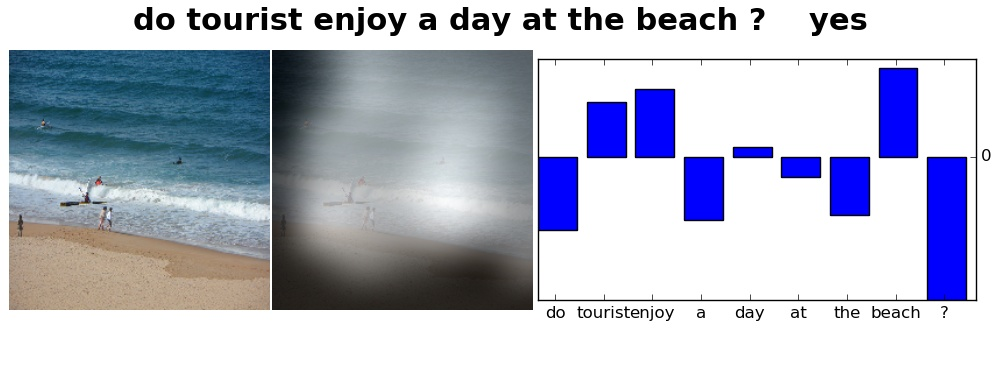
\includegraphics[width=0.5\textwidth]{figures/word_atten/COCO_val2014_000000540932_5409320.jpg}
  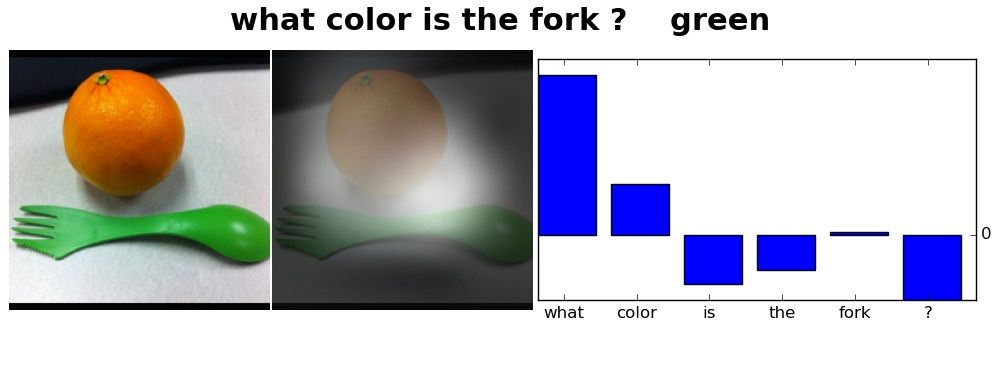
\includegraphics[width=0.5\textwidth]{figures/word_atten/COCO_val2014_000000563730_5637302.jpg}\\
  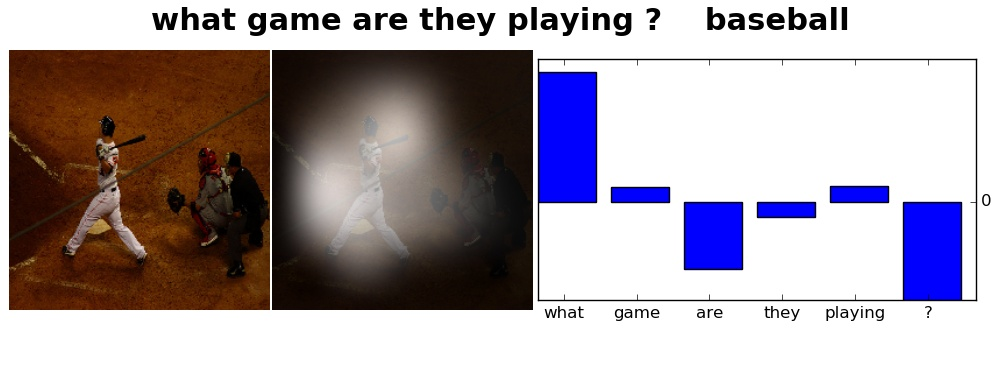
\includegraphics[width=0.5\textwidth]{figures/word_atten/COCO_val2014_000000576875_5768752.jpg}
  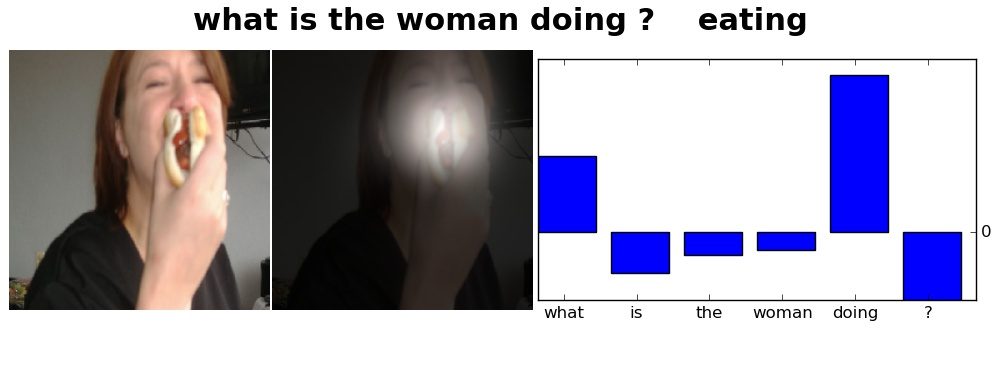
\includegraphics[width=0.5\textwidth]{figures/word_atten/COCO_val2014_000000567340_5673401.jpg}
\vspace{-0.3in}
\caption{
Visualization of the original image (left), the spatial attention weights $W_{att}$ in the first hop (middle) and one correlation vector from the correlation matrix $C$ for the location with highest attention weight in the SMem-VQA Two-Hop model on the VQA dataset.
Higher values in the correlation  vector indicate  stronger correlation of that word with the chosen location's image features.}
\label{fig:VQA_hop1Atten_wordAtten}
\vspace{-0.15in}
\end{figure*}




 






\label{sec:conclusion}
We introduce a novel neural network architecture, the Synchronized Spectral CNN (SyncSpecCNN), for semantic annotation on 3D shape graphs. To share coefficients and conduct multi-scale analysis in different parts of a single shape graph, we introduce a spectral parametrization of dilated convolutional kernels. To allow parameter sharing across related but different shapes that may be represented by very different graphs, we introduce a spectral transformer network to synchronize different spectral domains. The effectiveness of different components in our network is validated through extensive experiments. Jointly these contributions lead to state-of-the-art performance on various semantic annotation tasks including 3D shape part segmentation and 3D keypoint prediction.

\clearpage
\clearpage

{\small
\bibliographystyle{ieee}
\bibliography{egbib}
}

\end{document}
